\documentclass{article}
\title{Nechyba Ch.17 风险存在时的选择与市场}
\author{Dawei Wang}
\date{\today}
\usepackage{ctex}
\usepackage{amsmath}
\usepackage{amssymb}
\usepackage{graphicx} %插入图片的宏包
\usepackage{float} %设置图片浮动位置的宏包
\usepackage{subfigure} %插入多图时用子图显示的宏包
\begin{document}
	\maketitle
    偏好与约束的组合决定选择,不同的人对风险有不同的态度(或者偏好),市场的价格决定了个人处理他们面临的风险时所作出的选择。

\section{风险存在时选择的直观模型}

\subsection{涉及钱的风险选择}

对个体的效用像一个单一要素生产过程那样建模,其中生产要素是年消费而产出是“效用”。

\begin{figure}[H] %H为当前位置,!htb为忽略美学标准,htbp为浮动图形
	\centering %图片居中^{}
	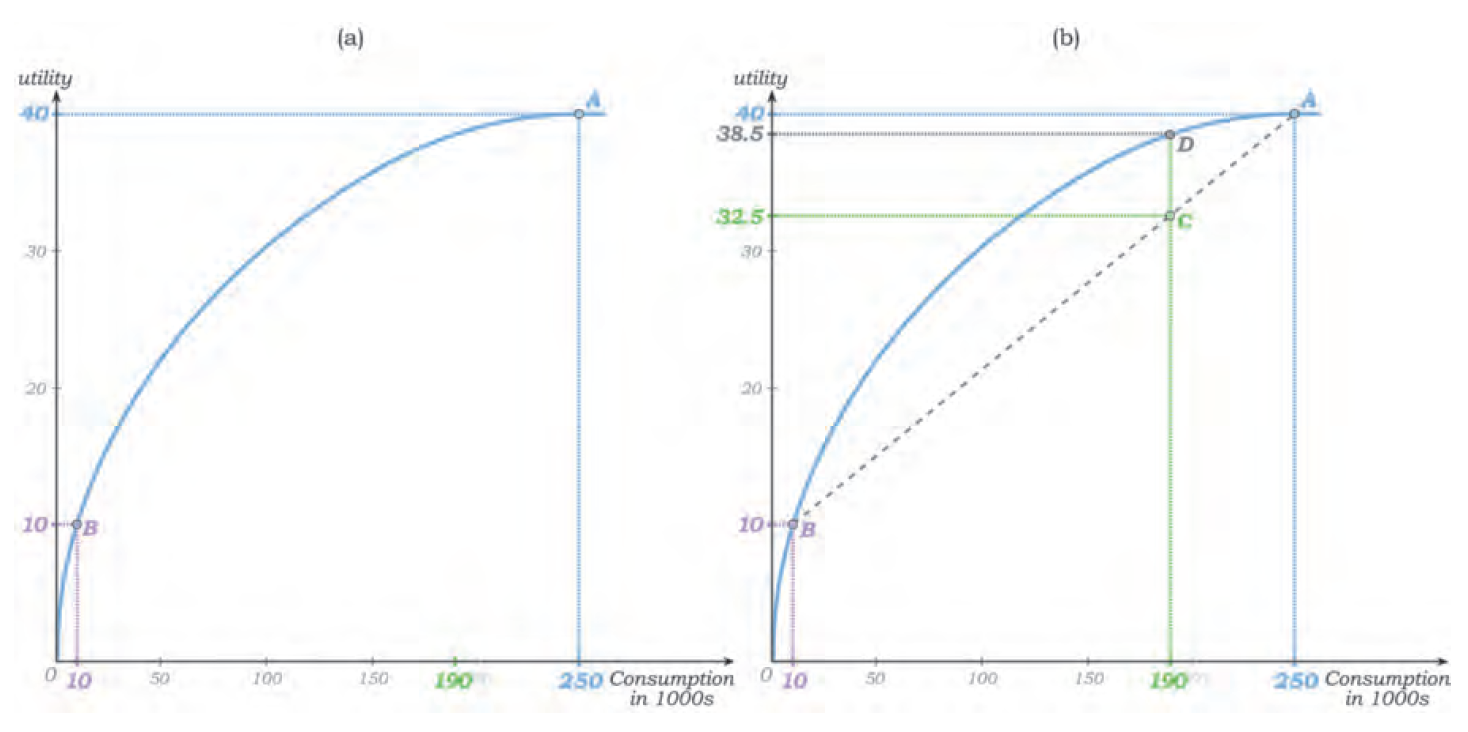
\includegraphics[width=1\textwidth]{17_1} %插入图片,[]中设置图片大小,{}中是图片文件名
	\caption{Relation of “Utility” to “Consumption”} %最终文档中希望显示的图片标题
	\label{Fig.main2} %用于文内引用的标签
\end{figure}

上图所示的“生产边界”意味着递减的边际效用。简单起见,我们把所有的消费品加总起来当成一个复合商品。

\hspace*{\fill}

对风险的不同态度

一个风险厌恶的人在一个赌局中期望值的效用总是高于这个赌局的期望效用。

\begin{figure}[H] %H为当前位置,!htb为忽略美学标准,htbp为浮动图形
	\centering %图片居中^{}
	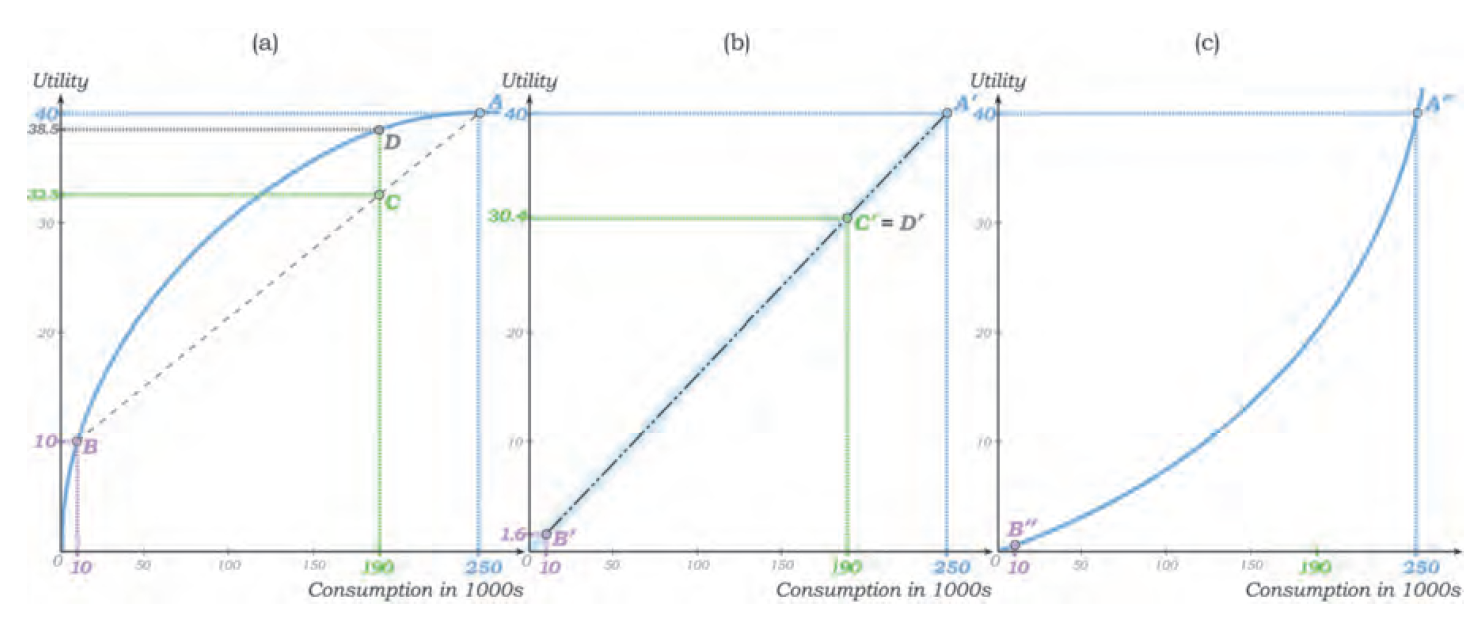
\includegraphics[width=1\textwidth]{17_2} %插入图片,[]中设置图片大小,{}中是图片文件名
	\caption{Risk Aversion, Risk Neutrality, and Risk Loving} %最终文档中希望显示的图片标题
	\label{Fig.main3} %用于文内引用的标签
\end{figure}

\hspace*{\fill}

确定性等价与风险溢价

某个人为了不参与赌局愿意(确定地)接受的最小数量,称作赌局的确定性等价(certainty equivalent of the gamble)。一个赌局的风险溢价(risk premium)是一个赌局的期望值与它的确定性等价的差。

\hspace*{\fill}

“精算公平”保险市场

一个保险合同或保单由两部分组成:一部分是保费,是消费者在知道ta所面临的结果是什么的时候同意支付的金额;另一部分是保险收益,即被保险人在最终面对“坏”结果时有权限享有的金额。

假定存在一个对个人所面对的风险有着完全信息的竞争性保险行业。在完全竞争下,每个保险公司将会得到零净利润,假定“坏”结果的概率是$ \delta $,收益为b,保费为p,那么在长期均衡中$ b=p/\delta $,这种保险合同被称为精算公平(actuarily fair)。

风险厌恶者在精算公平的保险市场中将会选择全保。在非精算公平保险市场中不会选择全保。

\subsection{涉及多重“世界状态”的风险选择}

简单模型具有一定的局限性,只有在处于两种世界状态的人用同一效用函数表示钱带来的效用时才是合理的。

当消费者被赋予不同数量的两种商品而没有任何其他收入来源时这个一般均衡模型与一个两商品世界的消费者选择模型有着很强的相似性。

\begin{figure}[H] %H为当前位置,!htb为忽略美学标准,htbp为浮动图形
	\centering %图片居中
	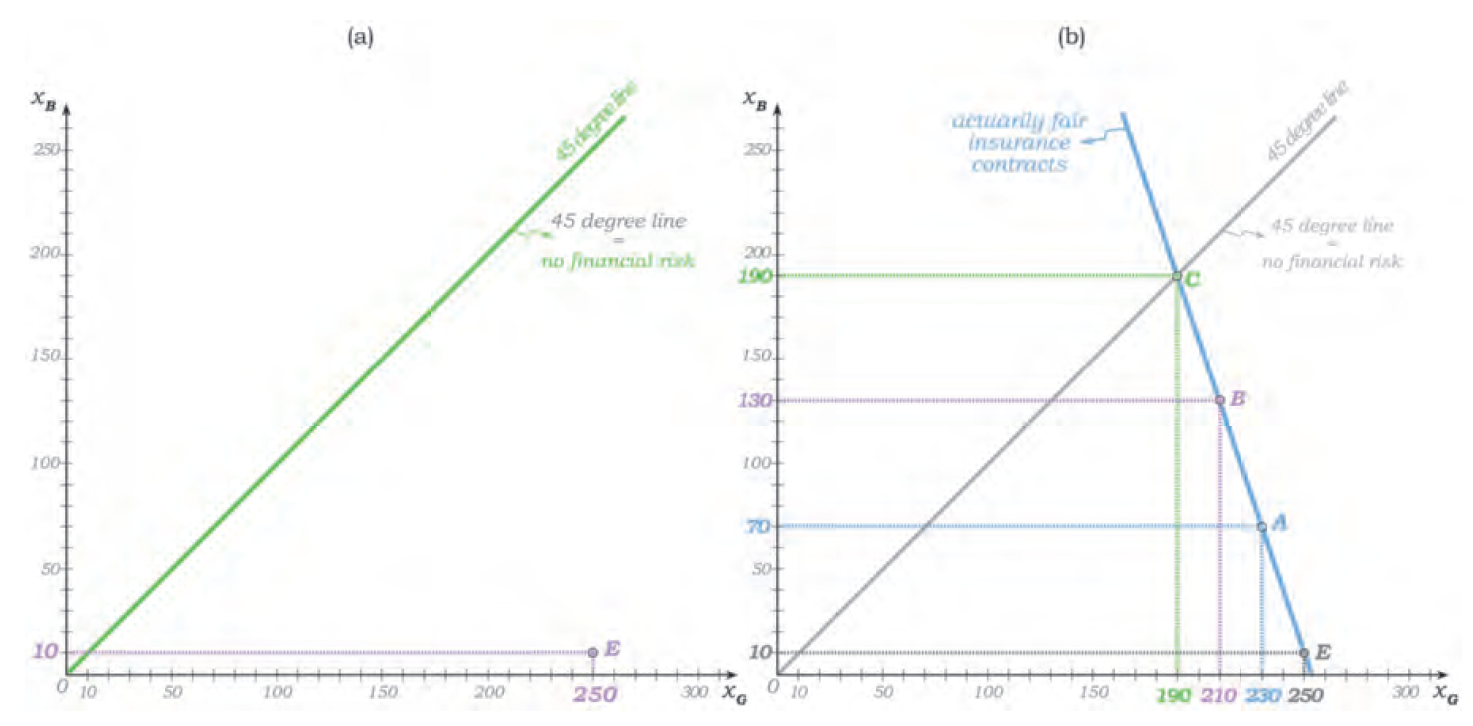
\includegraphics[width=1\textwidth]{17_3} %插入图片,[]中设置图片大小,{}中是图片文件名
	\caption{Consumption in Different “States”} %最终文档中希望显示的图片标题
	\label{Fig.main4} %用于文内引用的标签
\end{figure}

把好状态下的消费(记为$ x_G $)放在横轴且把坏状态下的消费(记为$ x_B $)放在纵轴。其中45度线表示无财务风险,所有45度线以下的保单表示该保单中消费者没有全保,从而使得坏状态比在好状态下消费要少些;而45度线以上的保单导致了“过度保险”,在该保单中消费者在坏状态下的消费比在好状态下的消费要多。

\hspace*{\fill}

当只有钱重要时的无差异曲线

仅当钱是重要的时,任何风险厌恶的消费者在给定所有的精算公平保险合同的选择时都会选择对风险全保,因此最优的无差异曲线与预算集的切点将会位于45度线上。

如果记坏状态的概率为$ \delta $,好状态的概率为$ (1-\delta) $,精算公平保险合同的预算约束的斜率将为$ -(1-\delta)/\delta $。对于当两种“世界状态”没有差别,当只有钱重要的特殊情况,这意味着风险厌恶的消费者的边际替代率沿着45度线为$ (1-\delta)/\delta $。

\begin{figure}[H] %H为当前位置,!htb为忽略美学标准,htbp为浮动图形
	\centering %图片居中
	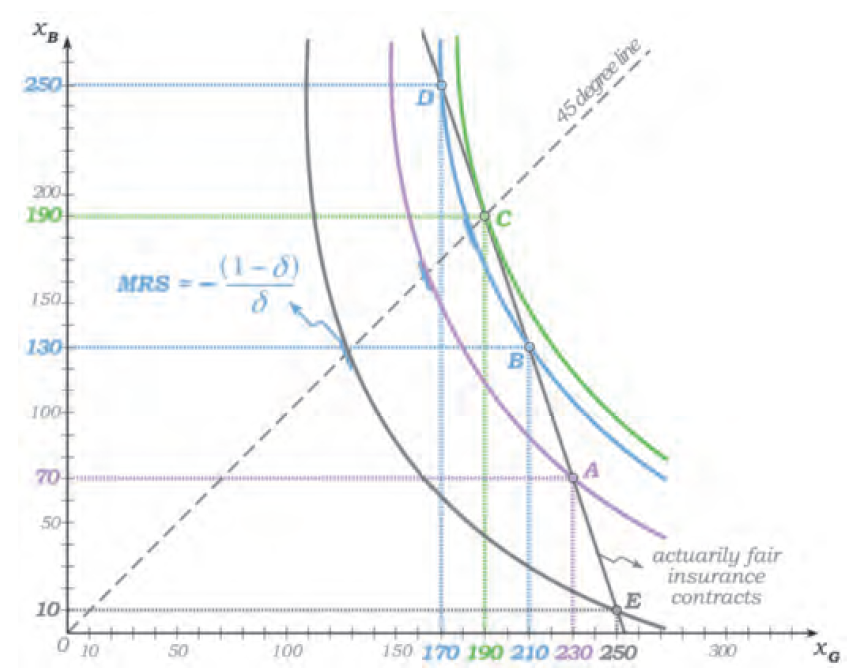
\includegraphics[width=1\textwidth]{17_4} %插入图片,[]中设置图片大小,{}中是图片文件名
	\caption{Risk-Averse Indifference Curves when “Only Money Matters”
		actuarily} %最终文档中希望显示的图片标题
	\label{Fig.main5} %用于文内引用的标签
\end{figure}

凸性意味着当我们有像B和D这样的极端束时,那些束的平均被偏好(如C)。因为沿着经过B,C和D的线的期望消费不变,这意味着只要赌局的期望效用值不变,更少的风险(如C)要好于更多的风险(如B和D)。但这也正是风险厌恶的定义。从而,当这个模型中无差异曲线满足凸性时,消费者是风险厌恶的。

以前没有风险的消费者模型中,束$ (x_1,x_2) $是$ x_1 $单位第一种商品与$ x_2 $单位的第二种商品组成的束。零一方面,在我们有风险的模型中,点$ (x_G,x_B) $表示两个永远也不会一起消费的分离的消费水平。如果遇到“好状态”,$ x_G $是可得的消费量;如果遇到“坏状态”,$ x_B $是可得的消费量。

\hspace*{\fill}

当“状态”不同时的无差异曲线与选择集

如果在“好”状态和“坏状态”之间没有内在差别,对风险厌恶的消费者的无差异曲线将有通常的凸性并且沿着45度线的MRS等于$ (1-\delta)/\delta $。

\begin{figure}[H] %H为当前位置,!htb为忽略美学标准,htbp为浮动图形
	\centering %图片居中
	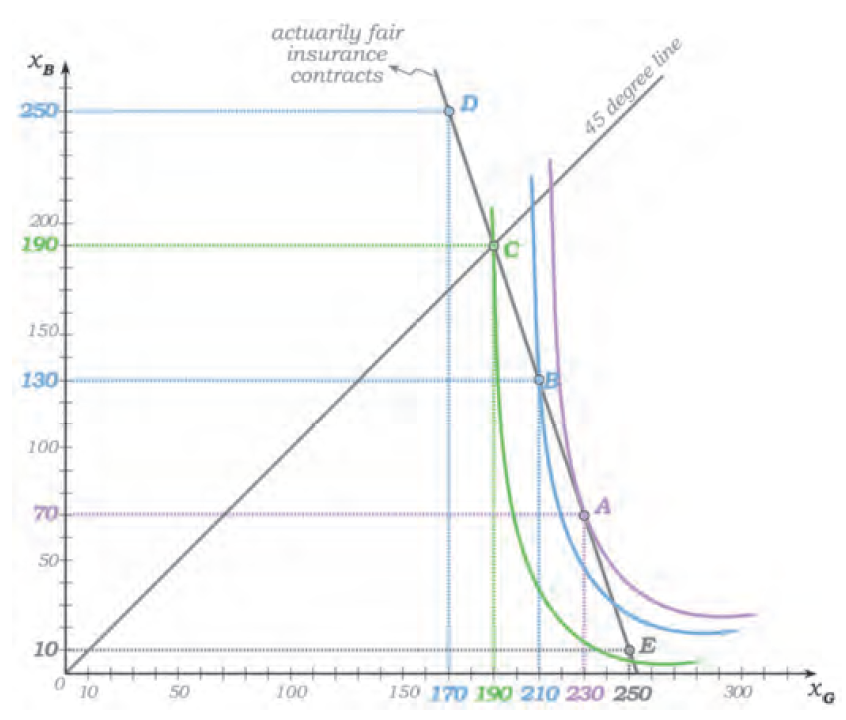
\includegraphics[width=1\textwidth]{17_5} %插入图片,[]中设置图片大小,{}中是图片文件名
	\caption{Insurance Choice when Utility Is “State-Dependent”} %最终文档中希望显示的图片标题
	\label{Fig.main6} %用于文内引用的标签
\end{figure}

尽管风险厌恶在一个只有钱重要的“状态独立”的模型中意味着全保,但这说明了在“状态相关”模型中风险厌恶与低于全保相一致。因此,当我们观察到一个个体没有全保时,它可能是由于保险市场不是精算公平的,也可能因为该个体有状态相关效用。

\subsection{不确定性下的一般均衡}

没有总体风险的有效性

无总体风险:在总体上,经济生产相同的东西而不管哪个状态发生。

\hspace*{\fill}

假定交易双方的效用函数都是“状态独立”的。因此沿着45度线,我们无差异曲线的边际替代率等于$ (1-\delta)/\delta $。

\begin{figure}[H] %H为当前位置,!htb为忽略美学标准,htbp为浮动图形
	\centering %图片居中
	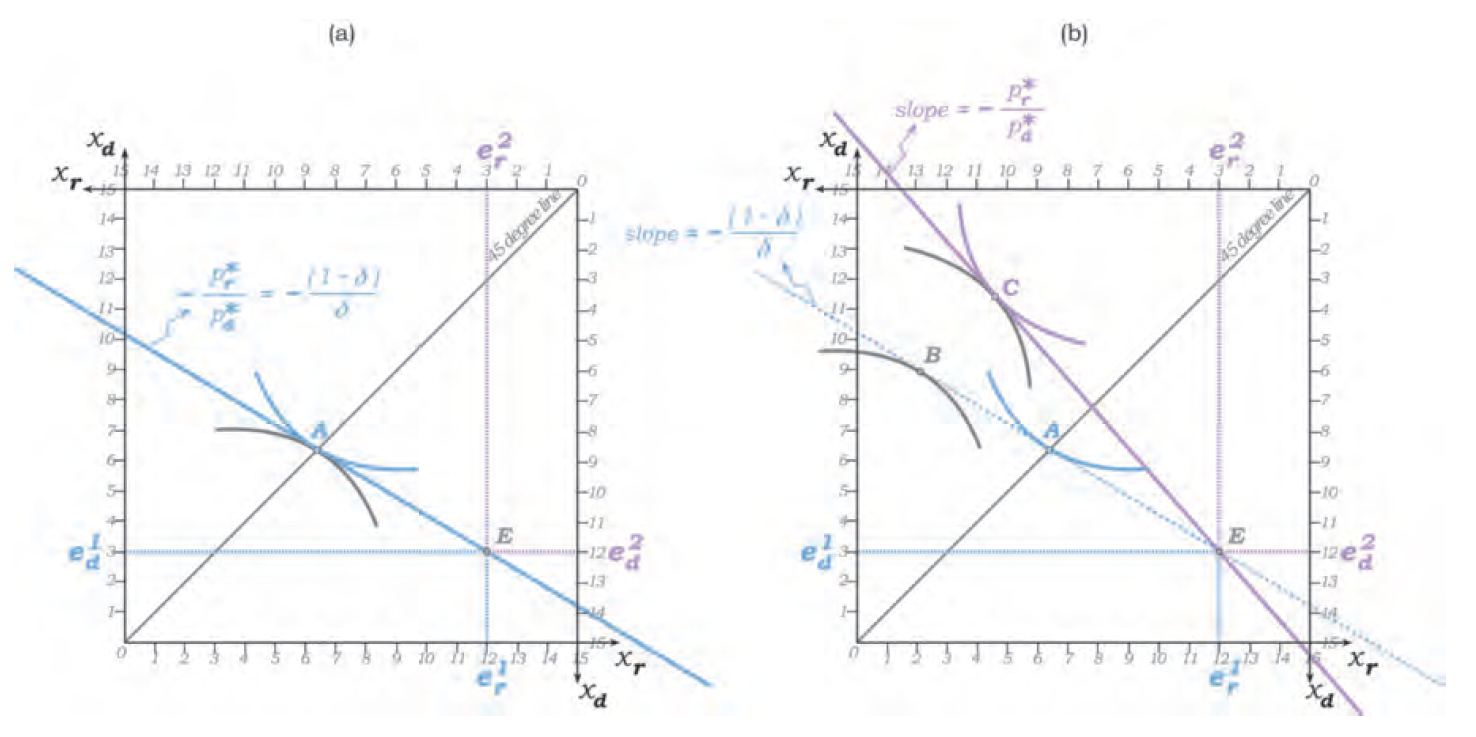
\includegraphics[width=1\textwidth]{17_6} %插入图片,[]中设置图片大小,{}中是图片文件名
	\caption{Equilibrium Contracts with No Aggregate Risk} %最终文档中希望显示的图片标题
	\label{Fig.main7} %用于文内引用的标签
\end{figure}

为找到将执行的合同的竞争性均衡条款$ p_r^*/p_d^* $,我们需要找到条款来构造一条通过禀赋点的斜率为$ (1-\delta)/\delta $的预算线。在偏好不是状态相关时,我们合同的均衡条款有着“精算公平”的特征。

继续假设交易的一方的偏好是“状态独立”的,但另一人不是状态独立的,此时契约曲线不再是45度线。

\hspace*{\fill}

引入总体风险

当总体存在风险时,Edgeworth图不再是正方形。

若交易双方是状态独立的,我们就知道沿着45度线的边际替代率等于$ (1-\delta)/\delta $。但这意味着我们无法在一个竞争性均衡合同中有$ p_r^*/p_d^*=(1-\delta)/\delta $的精算公平条款

\begin{figure}[H] %H为当前位置,!htb为忽略美学标准,htbp为浮动图形
	\centering %图片居中
	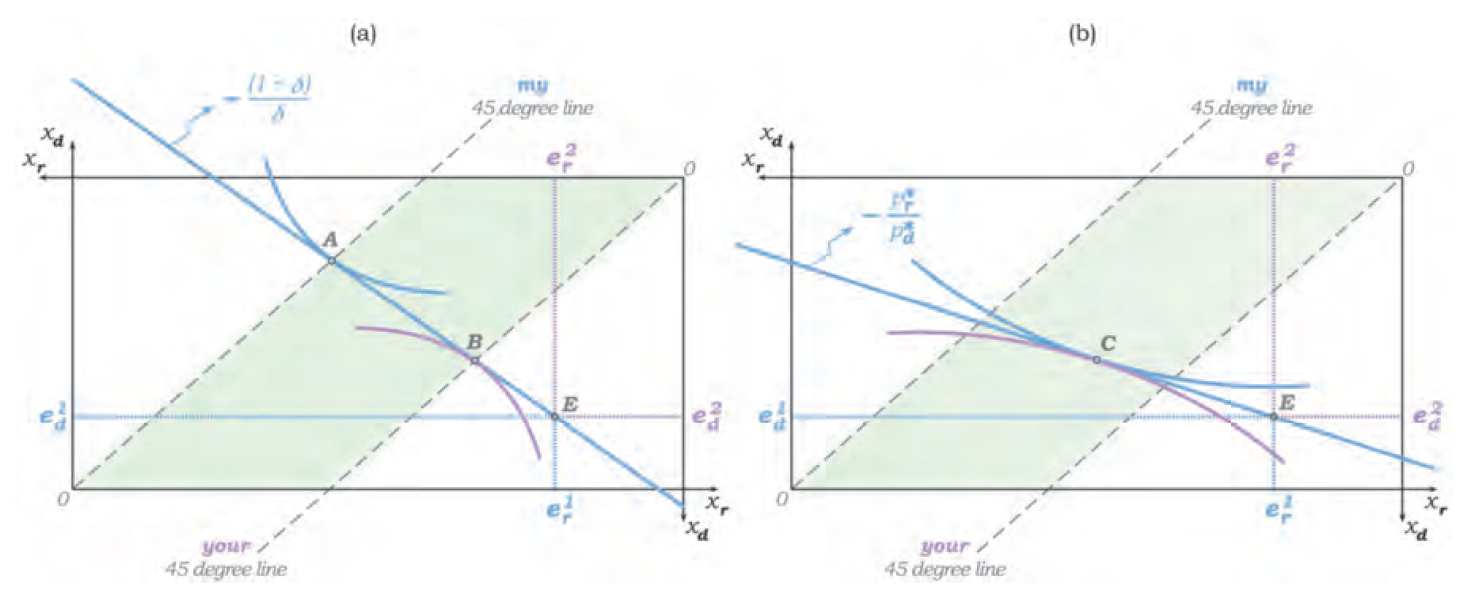
\includegraphics[width=1\textwidth]{17_7} %插入图片,[]中设置图片大小,{}中是图片文件名
	\caption{Equilibrium with Aggregate Risk} %最终文档中希望显示的图片标题
	\label{Fig.main8} %用于文内引用的标签
\end{figure}

现在使得交易双方的无差异曲线能够彼此相切的唯一区域位于两条45度线之间。从而我们断定$ p_r^*/p_d^* $一定要比$ (1-\delta)/\delta $小。

这个结果可以一般化为:当存在总体风险时,“坏”状态下的商品在总体风险越大的情况下有着相对更高的价值。

\section{风险存在时的数学分析}

\subsection{效用与期望效用}

假定坏的情况发生的概率为$ \delta $且状态独立,则风险存在时的效用函数为:

\[
U(x_G,x_B)=\delta u(x_B)+(1-\delta)u(x_G)
\]

如果把效用函数u(x)理解为衡量消费的效用,上式就是一个简单的“期望效用”的效用函数。

采取期望效用形式并且表示一个消费者对风险赌局的潜在的无差异曲线的效用函数$ U(x_G,x_B) $被称为von Neumann-Morgenstern expected utility
function。

\hspace*{\fill}

风险厌恶与凹性

一个个体是风险厌恶的当且仅当这个赌局的期望值的效用比这个赌局的期望效用更高;意即,当且仅当$ u(E(x))>U(x_G,x_B) $。这可以展开为:

\[
u(\delta x_B+(1-\delta)x_G)=u(E(x))>U(x_G,x_B)=\delta u(x_B)+(1-\delta)u(x_G)
\]

一个凹函数可以被定义为一个函数f,使得对所有$ x_1\ne x_2 $以及所有介于0和1之间的$ \delta $,有

\[
f(\delta x_1+(1-\delta)x_2)>\delta f(x_1)+(1-\delta)x_2
\]

个体的风险厌恶意味着任何一个使得我们能用期望效用函数来表示这样一个偏好的函数一定是凹的。因此,不是假定u(x)的凹性来得到风险厌恶的偏好,而是如果对风险厌恶并且u可以被用来以期望效用的形式表示对$ (x_G,x_B) $的无差异曲线,我们推出u(x)一定是凹的。

\hspace*{\fill}

u(x)的凹性与偏好的凸性

当建立消费者理论时的“平均优于极端”指的是如果一个消费者在两个束之间无差异,ta将偏好那两个束的任意加权平均胜于开始的任何一个更加极端的束。若ta对束$ (x_G,x_B) $的无差异曲线用期望效用函数$ U(x_G,x_B)=\delta u(x_B)+(1-\delta)u(x_G) $来描述。现取存在束$ (x_G^1,x_B^1),(x_G^2,x_B^2) $使得

\[
U(x_G^1,x_B^1)=U(x_G^2,x_B^2)=\overline{U}
\]

考虑这两个结果的一个加权平均$ (x_G^3,x_B^3) $;也就是对介于0和1之间的某个$ \alpha $,考虑$ (x_G^3,x_B^3) $使得

\[
x_G^3=\alpha x_G^2+(1-\alpha)x_G^1\enspace and\enspace x_B^3=\alpha x_B^2+(1-\alpha)x_B^1
\]

\begin{equation*}
	\begin{split}
	U(x_G^3,x_B^3)&=\delta u(x_B^3)+(1-\delta)u(x_G^3)\\
	&>\delta[\alpha u(x_B^2)+(1-\alpha)u(x_B^1)]+(1-\delta)[\alpha u(x_G^2)+(1-\alpha)u(x_G^1)]\\
	&=\alpha U(x_G^2,x_B^2)+(1-\alpha)U(x_G^1,x_B^1)\\
	&=\alpha\overline{U}+(1-\alpha)\overline{U}=\overline{U}
	\end{split}	
\end{equation*}

从而现在已经证明了风险厌恶意味着u(x)的凹性和是u(x)的凹性意味着对结果$ (x_G,x_B) $的无差异曲线的凸性。

\hspace*{\fill}

确定性等价与风险溢价 

一个赌局的确定性等价(certainty equivalent)是一个人为了不参与这个赌局最少要接受的量。

\hspace*{\fill}

精算保险市场

保险由两部分组成:坏的情况发生时的保险收益b(insurance benefit)、保费(premium)p,这意味着好的情况下的收入为$ (x_G-p) $,坏的情况下的收入为$ (x_B+b-p) $。

假定投保者被提供精算公平的保单全集;也就是那些不改变其期望收入但是降低了风险的政策,因此:
\[
\delta(b-p)=(1-\delta)p
\]
得:
\[
b=p/\delta
\]

其从一个精算公平政策(b,p)得到的期望效用是
\[
U(x_G,x_B)=\delta u(x_B+b-p)+(1-\delta)u(x_G-p)\enspace s.t.\enspace b=\frac{p}{\delta}
\]

在面对一个精算公平保险市场时,这个模型中一个风险厌恶的人总是选择全保,也就是不管什么状态发生都能确保收入是一样的。二者都为:

\[
x=\delta x_B+(1-\delta)x_G
\]

\subsection{涉及多种“世界状态”的风险选择}

不同“世界状态”下的消费模型

\[
U(x_G,x_B)=\delta u_B(x_B)+u_G(x_G)
\]

这与前面的期望效用函数的唯一差别是在两个不同世界状态下用来度量效用的函数采取不同形式,在前面,当时世界状态与个人对消费的感觉无关时,一个单一函数u(x)被用在期望效用函数$ U(x_G,x_B) $中。

精算公平保险下的选择集

设禀赋点为$ (e_G,e_B) $,此时精算公平保险下的选择集为:

\[
\delta e_B+(1-\delta)e_G=\delta x_B+(1-\delta)x_G
\]

\hspace*{\fill}

对精算公平保险合同的选择

\[
\max\limits_{x_G,x_B} U(x_G,x_B)=\delta u_B(x_B)+(1-\delta)u_G(x_G)
\]

\[
s.t.\enspace \delta e_B+(1-\delta)e_G=\delta x_B+(1-\delta)x_G
\]

\subsection{风险下的一般均衡}

保险合同表示一个状态下卖出状态相机消费来购买另一个状态下的相机消费的特定方式。

允许两个消费者对每个状态实际发生的可能性有着不同信念,消费者1对状态1设置的概率是$\delta$,消费者2对状态1设置的概率是$\gamma$。

无总体风险意味着$ e^1_1+e^2_1=e^1_2+e^2_2 $,并且我们每个人都知道事故发生的机会意味着$ \delta=\gamma $

\hspace*{\fill}

引入对风险的不同信念

\[
\delta\ne\gamma
\]

引入总体风险

\[
e^1_1+e^2_1\ne e^1_2+e^2_2
\]




\end{document}